\section{Evolving Paradigms of Audio Interaction and Discussion}
\label{sec:interaction_paradigms}


\begin{figure}[!t]
    \centering
    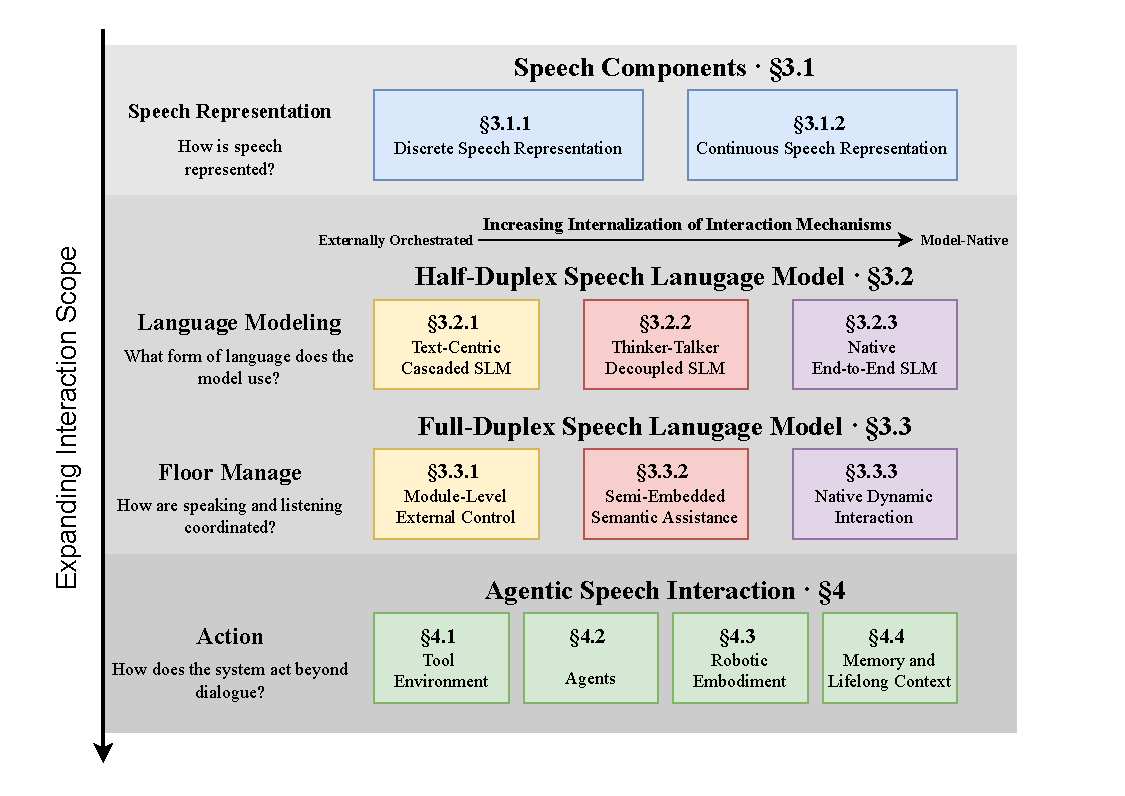
\includegraphics[width=\textwidth,height=0.78\textheight,keepaspectratio]{figures/Taxonomy.pdf}
    \caption{The taxonomy of audio interaction.}
    \label{fig:audio-interaction-taxonomy}
\end{figure}

% Understanding the development of speech interaction requires distinguishing the interaction functions a system supports from the mechanisms that realize them. Figure~\ref{fig:interaction_taxonomy} organizes this distinction along two directions. Vertically, the roadmap expands from speech representation to language interaction, conversational timing, and action beyond dialogue. Horizontally, the taxonomy examines how language interaction and timing control are incorporated into the core interaction model. We refer to this incorporation as the \emph{internalization of interaction mechanisms}. It concerns the role of the core model in a particular interaction function, rather than the number of components or whether the entire system is jointly trained. The roadmap describes an expansion of analytical scope, not a sequence that every system must follow.

Figure~\ref{fig:audio-interaction-taxonomy} distinguishes the scope of interaction from how individual mechanisms are implemented. Vertically, the roadmap begins with speech representation as the technical foundation and extends to action beyond dialogue. Horizontally, we compare designs in language modeling and floor management by the extent to which the core interaction model handles the relevant mechanism. We refer to this organizing principle as the \emph{internalization of interaction mechanisms}. The spectrum runs from externally orchestrated mechanisms to model-native capabilities, with intermediate designs dividing the work between external components and the core model. A system's position on this spectrum is assessed for each mechanism, regardless of its component count or whether the entire system is jointly trained.

\paragraph{Speech Representation: the foundation of speech interaction.}
The first question is how speech enters and leaves the model's representation space. Discrete tokens and continuous representations offer different ways to make acoustic signals available for computation and generation~\cite{DBLP:conf/acl/CuiYJMZWGK25}. Both can retain linguistic and acoustic information, with their usefulness depending on what is preserved, compressed, and made accessible to subsequent modeling. Section~\ref{sec:speech-components} therefore treats discrete and continuous representations as alternative foundations rather than successive levels of interaction intelligence. Representation determines what information is available; the following parts examine how that information participates in interaction.


\paragraph{Language Modeling: the form of language within the interaction model.}
With speech represented, the next concern is whether the core model conducts language interaction through text, speech, or a combination of both. Section~3.2 examines this question within half-duplex dialogue, where users and systems alternate speaking turns. In text-centric cascades, recognition and synthesis surround a text-based dialogue model. Thinker-Talker systems bring speech information directly into understanding, while replies remain organized around text and are realized by a separate speech generator. Native end-to-end speech models extend the role of speech representations into the modeling of both conversational input and output~\cite{}. These distinctions concern the model's medium of language interaction, not simply its output modality. Internalization here describes the extent to which speech participates in the core model's understanding and response formation. Auxiliary text may remain useful in native speech models, and streaming computation can operate within a turn-based interaction policy.

\paragraph{Timing: the coordination of speaking and listening.}
The form of language used by a model does not, by itself, determine how it coordinates with another speaker. Full-duplex interaction brings ongoing input and output into the same conversational process, requiring decisions about when to speak, continue listening, or adjust an unfolding response~\cite{DBLP:conf/emnlp/VeluriPYGG24}. Accordingly, Section~3.3 distinguishes module-level external control, semi-embedded semantic assistance, and native dynamic interaction based on where these decisions are made. Specifically, external controllers manage timing separately from the response model; semi-embedded mechanisms use the model's internal representations to inform control; and native mechanisms incorporate timing decisions into the model's ongoing generation. Here, internalization concerns conversational coordination rather than the use of speech as a language medium; native timing control need not eliminate external audio-processing or serving components. This distinction explains why a native speech model can remain turn-based, while an externally controlled system can support full-duplex behavior. The key distinction, therefore, lies in how conversational timing is determined, not simply how quickly speech is generated.

\paragraph{Action: extending interaction beyond dialogue.}
Agentic audio interaction expands the scope from exchanging utterances to acting on tasks and incorporating their consequences into subsequent interaction. In the outlook developed in Section~4, speech remains the primary interface between users and agents, while agents use tools, collaborate with other agents, act through robotic embodiments, and access persistent memory~\cite{}. These categories identify targets of action rather than levels of internalization, and a system may combine several of them. The extension concerns the relationship between spoken goals, agent actions, and environmental feedback. Speech connects users to this process throughout a task, allowing them to refine intentions and interpret outcomes. We distinguish existing mechanisms from the broader prospect of sustained collaboration; neither tool access nor full-duplex dialogue alone establishes this capability.

Taken together, the roadmap separates the expansion of interaction scope from the internalization of particular mechanisms. Language and timing need not be internalized to the same degree, and action capabilities can be built on either turn-based or full-duplex dialogue. Bringing a mechanism into the core model creates opportunities to learn its dependencies on conversational context, but its effectiveness still depends on representation, training, and execution~\cite{}. External components can retain advantages in controllability and independent optimization. The taxonomy thus supports comparison through what each design makes possible and what it leaves unresolved, rather than treating architectural integration as a universal measure of progress.


\begin{figure*}[tp]
  \centering
  \begin{adjustbox}{
    max totalsize={\textwidth}{0.90\textheight},
    center
  }
  \begin{tikzpicture}[
    taxonomy node/.style={
      draw=gray!65,
      rounded corners=2pt,
      inner sep=4pt,
      font=\scriptsize
    },
    taxonomy detail/.style={
      taxonomy node,
      text width=10.6cm,
      align=left
    },
    taxonomy topic/.style={
      taxonomy node,
      text width=2.4cm,
      align=center
    },
    taxonomy group/.style={
      taxonomy node,
      text width=2.1cm,
      align=center,
      font=\bfseries\scriptsize,
      execute at begin node={\hyphenpenalty=10000\relax}
    },
    taxonomy edge/.style={
      draw=gray!65,
      line width=0.4pt
    }
  ]

  % =========================================================
  % Speech Components
  % =========================================================

  \node[
    taxonomy detail,
    fill=brightlavender!12,
    anchor=north west
  ] (detail0) at (7.25,0) {
    \taxwork{HuBERT}{DBLP:journals/taslp/HsuBTLSM21};
    \taxwork{CosyVoice~2}{DBLP:journals/corr/abs-2412-10117};
    \taxwork{SoundStream}{DBLP:journals/taslp/ZeghidourLOST22};
    \taxwork{EnCodec}{DBLP:journals/tmlr/DefossezCSA23};
    \taxwork{WavTokenizer}{DBLP:conf/iclr/Ji00C0Z0C0LZY0J25};
    \taxwork{SpeechTokenizer}{DBLP:conf/iclr/ZhangZLZQ24};
    \taxwork{X-Codec}{DBLP:conf/aaai/YeSL00DKCPLGX25};
    \taxwork{Mimi}{DBLP:journals/corr/abs-2410-00037};
    \taxwork{DualCodec}{DBLP:conf/interspeech/LiLLHWWZ025}.
  };

  \node[
    taxonomy topic,
    fill=brightlavender!20,
    anchor=west
  ] (topic0) at (4.2,0 |- detail0.west) {
    Discrete Speech Representation
  };
  \draw[taxonomy edge] (topic0.east) -- (detail0.west);

  \node[
    taxonomy detail,
    fill=brightlavender!12,
    anchor=north west
  ] (detail1) at ($(detail0.south west)+(0,-0.2)$) {
    \taxwork{tGSLM}{DBLP:conf/emnlp/AlgayresANCSSD23};
    \taxwork{Spectron}{DBLP:conf/iclr/NachmaniLHSAMRS24};
    \taxwork{LauraGPT}{DBLP:journals/corr/abs-2310-04673};
    \taxwork{Mini-Omni}{DBLP:journals/corr/abs-2408-16725};
    \taxwork{SLAM-Omni}{DBLP:conf/acl/Chen0YLLXN00L0025};
    \taxwork{Flow-Omni}{DBLP:journals/corr/abs-2412-04917};
    \taxwork{Cont-SPT}{DBLP:conf/naacl/LiXSCK25};
    \taxwork{CALM}{DBLP:conf/iclr/RouardORZD26};
    \taxwork{HoliTok}{DBLP:journals/corr/abs-2605-29948}.
  };

  \node[
    taxonomy topic,
    fill=brightlavender!20,
    anchor=west
  ] (topic1) at (4.2,0 |- detail1.west) {
    Continuous Speech Representation
  };
  \draw[taxonomy edge] (topic1.east) -- (detail1.west);

  % =========================================================
  % Half-Duplex Interaction
  % =========================================================

  \node[
    taxonomy detail,
    fill=lightgreen!12,
    anchor=north west
  ] (detail2) at ($(detail1.south west)+(0,-0.4)$) {
    \taxwork{POMDP SDS}{DBLP:journals/pieee/YoungGTW13};
    \taxwork{SimpleTOD}{DBLP:conf/nips/Hosseini-AslMWY20};
    \taxwork{AudioGPT}{DBLP:conf/aaai/HuangLYSCYWHHLR24};
    \taxwork{ESPnet-SDS}{DBLP:conf/naacl/Arora0STCBFKTSS25};
    \taxwork{Eva}{DBLP:conf/ifaamas/QinZ25};
    \taxwork{LiveKit Agents}{livekitagentsdocs};
    \taxwork{Pipecat}{pipecatdocs};
    \taxwork{Schlangen \& Skantze}{DBLP:journals/dad/SchlangenS11};
    \taxwork{InproTK}{DBLP:conf/naacl/BaumannS12};
    \taxwork{Telecom Agent}{DBLP:journals/corr/abs-2508-04721};
    \taxwork{FireRedChat}{DBLP:journals/corr/abs-2509-06502};
    \taxwork{LTS-VoiceAgent}{DBLP:journals/corr/abs-2601-19952};
    \taxwork{DDTSR}{DBLP:journals/corr/abs-2602-23266}.
  };

  \node[
    taxonomy topic,
    fill=lightgreen!20,
    anchor=west
  ] (topic2) at (4.2,0 |- detail2.west) {
    Text-Centric Cascade
  };
  \draw[taxonomy edge] (topic2.east) -- (detail2.west);

  \node[
    taxonomy detail,
    fill=lightgreen!12,
    anchor=north west
  ] (detail3) at ($(detail2.south west)+(0,-0.2)$) {
    \taxwork{LLaMA-Omni}{DBLP:conf/iclr/FangGZMZ025};
    \taxwork{Freeze-Omni}{DBLP:conf/icml/WangLFZS000M25};
    \taxwork{MinMo}{DBLP:journals/corr/abs-2501-06282};
    \taxwork{Uni-MoE}{DBLP:journals/pami/LiJHWZLMZ25};
    \taxwork{Qwen2.5-Omni}{DBLP:journals/corr/abs-2503-20215};
    \taxwork{LLaMA-Omni~2}{DBLP:journals/corr/abs-2505-02625};
    \taxwork{SALMONN-omni}{DBLP:journals/corr/abs-2505-17060};
    \taxwork{Qwen3-Omni}{DBLP:journals/corr/abs-2509-17765};
    \taxwork{Uni-MoE-2.0-Omni}{DBLP:journals/corr/abs-2511-12609};
    \taxwork{Qwen3.5-Omni}{DBLP:journals/corr/abs-2604-15804}.
  };

  \node[
    taxonomy topic,
    fill=lightgreen!20,
    anchor=west
  ] (topic3) at (4.2,0 |- detail3.west) {
    Thinker--Talker Decoupling
  };
  \draw[taxonomy edge] (topic3.east) -- (detail3.west);

  \node[
    taxonomy detail,
    fill=lightgreen!12,
    anchor=north west
  ] (detail4) at ($(detail3.south west)+(0,-0.2)$) {
    \taxwork{SpeechGPT}{DBLP:conf/emnlp/ZhangLZZWZQ23};
    \taxwork{USDM}{DBLP:conf/nips/KimSJKKKLSOHYY24};
    \taxwork{Mini-Omni}{DBLP:journals/corr/abs-2408-16725};
    \taxwork{IntrinsicVoice}{DBLP:journals/corr/abs-2410-08035};
    \taxwork{GLM-4-Voice}{DBLP:journals/corr/abs-2412-02612};
    \taxwork{Flow-Omni}{DBLP:journals/corr/abs-2412-04917};
    \taxwork{SLAM-Omni}{DBLP:conf/acl/Chen0YLLXN00L0025};
    \taxwork{Baichuan-Audio}{DBLP:journals/corr/abs-2502-17239};
    \taxwork{Kimi-Audio}{DBLP:journals/corr/abs-2504-18425};
    \taxwork{VITA-Audio}{DBLP:journals/corr/abs-2505-03739};
    \taxwork{Step-Audio~2}{DBLP:journals/corr/abs-2507-16632};
    \taxwork{MOSS-Speech}{DBLP:conf/iclr/ZhaoXJWCJCLCWZC26}.
  };

  \node[
    taxonomy topic,
    fill=lightgreen!20,
    anchor=west
  ] (topic4) at (4.2,0 |- detail4.west) {
    Native End-to-End Interaction
  };
  \draw[taxonomy edge] (topic4.east) -- (detail4.west);

  % =========================================================
  % Full-Duplex Interaction
  % =========================================================

  \node[
    taxonomy detail,
    fill=lightyellow!12,
    anchor=north west
  ] (detail5) at ($(detail4.south west)+(0,-0.4)$) {
    \taxwork{TurnGPT}{DBLP:conf/emnlp/EkstedtS20};
    \taxwork{RC-TurnGPT}{DBLP:conf/acl/JiangES23};
    \taxwork{VAP}{DBLP:conf/interspeech/EkstedtS22};
    \taxwork{Next-Turn}{DBLP:journals/corr/abs-2606-18094};
    \taxwork{Easy Turn}{DBLP:journals/corr/abs-2509-23938};
    \taxwork{FastTurn}{DBLP:journals/corr/abs-2604-01897};
    \taxwork{FlexDuo}{DBLP:journals/corr/abs-2502-13472};
    \taxwork{FireRedChat}{DBLP:journals/corr/abs-2509-06502};
    \taxwork{SoulX-Duplug}{arXiv:2603.14877};
    \taxwork{SID}{DBLP:journals/corr/abs-2603-24144};
    \taxwork{X-Talk}{DBLP:journals/corr/abs-2512-18706}.
  };

  \node[
    taxonomy topic,
    fill=lightyellow!20,
    anchor=west
  ] (topic5) at (4.2,0 |- detail5.west) {
    Module-Level External Control
  };
  \draw[taxonomy edge] (topic5.east) -- (detail5.west);

  \node[
    taxonomy detail,
    fill=lightyellow!12,
    anchor=north west
  ] (detail6) at ($(detail5.south west)+(0,-0.2)$) {
    \taxwork{Freeze-Omni}{DBLP:conf/icml/WangLFZS000M25};
    \taxwork{MinMo}{DBLP:journals/corr/abs-2501-06282};
    \taxwork{BC head}{DBLP:journals/corr/abs-2609-29418};
    \taxwork{VITA}{DBLP:journals/corr/abs-2408-05211}.
  };

  \node[
    taxonomy topic,
    fill=lightyellow!20,
    anchor=west
  ] (topic6) at (4.2,0 |- detail6.west) {
    Semi-Embedded Semantic Assistance
  };
  \draw[taxonomy edge] (topic6.east) -- (detail6.west);

  \node[
    taxonomy detail,
    fill=lightyellow!12,
    anchor=north west
  ] (detail7) at ($(detail6.south west)+(0,-0.2)$) {
    \taxwork{dGSLM}{DBLP:journals/tacl/NguyenKCAHETASM23};
    \taxwork{LSLM}{DBLP:conf/aaai/MaSDC0WW025};
    \taxwork{Moshi}{DBLP:journals/corr/abs-2410-00037};
    \taxwork{SyncLLM}{DBLP:conf/emnlp/VeluriPYGG24};
    \taxwork{OmniFlatten}{DBLP:conf/acl/ZhangCDCWZLYTDZ25};
    \taxwork{NTPP}{DBLP:journals/corr/abs-2506-00975};
    \taxwork{F-Actor}{DBLP:journals/corr/abs-2601-11329};
    \taxwork{DuplexCascade}{DBLP:journals/corr/abs-2603-09180};
    \taxwork{Raon-SpeechChat}{DBLP:journals/corr/abs-2605-23912};
    \taxwork{SALMONN-omni}{DBLP:journals/corr/abs-2505-17060};
    \taxwork{MiniCPM-o~4.5}{DBLP:journals/corr/abs-2604-27393};
    \taxwork{DuplexOmni}{DBLP:journals/corr/abs-2606-09186};
    \taxwork{BayLing-Duplex}{DBLP:journals/corr/abs-2606-14528};
    \taxwork{Lychee-FD}{DBLP:conf/acl/LiuZLTJCZMXHHLZ26};
    \taxwork{Realtime-Venus}{DBLP:journals/corr/abs-2609-13814};
    \taxwork{AdaptDuplex}{DBLP:journals/corr/abs-2609-29217};
    \taxwork{MultiTalk}{DBLP:journals/corr/abs-2609-36903};
    \taxwork{D2}{arXiv:2610.17124}.
  };

  \node[
    taxonomy topic,
    fill=lightyellow!20,
    anchor=west
  ] (topic7) at (4.2,0 |- detail7.west) {
    Native Dynamic Interaction
  };
  \draw[taxonomy edge] (topic7.east) -- (detail7.west);

  % =========================================================
  % Agentic Interaction
  % =========================================================

  \node[
    taxonomy detail,
    fill=paleblue!12,
    anchor=north west
  ] (detail8) at ($(detail7.south west)+(0,-0.4)$) {
    \taxwork{Spoken Function Calling}{DBLP:journals/corr/abs-2608-05126};
    \taxwork{Stream RAG}{DBLP:journals/corr/abs-2510-02044};
    \taxwork{Heard Enough to Act}{WEB:arxiv/2610.34653};
    \taxwork{SIA}{DBLP:journals/corr/abs-2605-13360};
    \taxwork{Gander}{DBLP:journals/corr/abs-2609-08977};
    \taxwork{StepAudio~3 Realtime}{WEB:arxiv/2609.14005};
    \taxwork{Qwen-Audio-Agent}{DBLP:journals/corr/abs-2609-25195};
    \taxwork{DuplexAgent-RSI}{WEB:arxiv/2610.11299};
    \taxwork{MoshiRAG}{tool_chien2026moshirag};
    \taxwork{PACE}{DBLP:journals/corr/abs-2608-07631};
    \taxwork{$\tau$-Voice}{tool_ray2026tauvoice};
    \taxwork{Qwen3.5-Omni}{DBLP:journals/corr/abs-2604-15804};
    \taxwork{VoiceChat}{DBLP:journals/corr/abs-2609-21967};
    \taxwork{DuplexSLA}{DBLP:journals/corr/abs-2605-20755};
    \taxwork{Frontend--Backend}{DBLP:journals/corr/abs-2609-19334};
    \taxwork{SALMONN-duo}{DBLP:journals/corr/abs-2609-34247};
    \taxwork{VoxMind}{DBLP:conf/acl/LiangCJCJLZPLZ26};
    \taxwork{SpeechGym}{DBLP:journals/corr/abs-2608-26432}.
  };

  \node[
    taxonomy topic,
    fill=paleblue!20,
    anchor=west
  ] (topic8) at (4.2,0 |- detail8.west) {
    Tool Environment
  };
  \draw[taxonomy edge] (topic8.east) -- (detail8.west);

  \node[
    taxonomy detail,
    fill=paleblue!12,
    anchor=north west
  ] (detail9) at ($(detail8.south west)+(0,-0.2)$) {
    \taxwork{SpeechAgents}{DBLP:journals/corr/abs-2401-03945};
    \taxwork{Interaction Models}{WEB:thinkingmachines/interaction-models};
    \taxwork{SALMONN-duo}{DBLP:journals/corr/abs-2609-34247};
    \taxwork{Gander}{DBLP:journals/corr/abs-2609-08977};
    \taxwork{VoxMind}{DBLP:conf/acl/LiangCJCJLZPLZ26};
    \taxwork{Qwen-Audio-Agent}{DBLP:journals/corr/abs-2609-25195};
    \taxwork{AdaptDuplex}{DBLP:journals/corr/abs-2609-29217};
    \taxwork{Jarvis}{WEB:arxiv/2610.23804}.
  };

  \node[
    taxonomy topic,
    fill=paleblue!20,
    anchor=west
  ] (topic9) at (4.2,0 |- detail9.west) {
    Agents
  };
  \draw[taxonomy edge] (topic9.east) -- (detail9.west);

  \node[
    taxonomy detail,
    fill=paleblue!12,
    anchor=north west
  ] (detail10) at ($(detail9.south west)+(0,-0.2)$) {
    \taxwork{Multimodal SR for Embodied Agents}{emb_chang2023};
    \taxwork{Multimodal Human--Autonomous Interaction}{emb_nwankwo2024};
    \taxwork{NMM-HRI}{emb_lai2025nmm};
    \taxwork{VLAS}{emb_zhao2025vlas};
    \taxwork{RoboOmni}{emb_wang2025roboomni};
    \taxwork{KnowNo}{emb_ren2023knowno};
    \taxwork{Interactive Language}{emb_lynch2022interactive};
    \taxwork{YAY Robot}{emb_shi2024yay};
    \taxwork{Incremental Language Understanding}{emb_abrams2025incremental};
    \taxwork{HEAR}{emb_nie2026hear};
    \taxwork{ELLSA}{emb_wang2026ellsa};
    \taxwork{VITA-E}{emb_liu2025vitae};
    \taxwork{MIRA}{emb_lin2026mira};
    \taxwork{Pepper LLM Framework}{emb_studerus2026pepper}.
  };

  \node[
    taxonomy topic,
    fill=paleblue!20,
    anchor=west
  ] (topic10) at (4.2,0 |- detail10.west) {
    Robotic Embodiment
  };
  \draw[taxonomy edge] (topic10.east) -- (detail10.west);

  \node[
    taxonomy detail,
    fill=paleblue!12,
    anchor=north west
  ] (detail11) at ($(detail10.south west)+(0,-0.2)$) {
    \taxwork{EgoMem}{DBLP:journals/corr/abs-2509-11914};
    \taxwork{VoiceMem}{DBLP:journals/corr/abs-2608-26005};
    \taxwork{VoiceTrace}{DBLP:journals/corr/abs-2609-18521};
    \taxwork{SpeakerMem-R1}{DBLP:journals/corr/abs-2609-26780};
    \taxwork{VoxPolyMem}{jia2026voxpolymem};
    \taxwork{Zep}{DBLP:journals/corr/abs-2501-13956};
    \taxwork{BELIEFMEM}{meng-etal-2026-beliefmem};
    \taxwork{APEX-MEM}{DBLP:conf/acl/BanerjeeMSMC26};
    \taxwork{TSHMem}{xu-etal-2026-tshmem};
    \taxwork{Voice Memory for Agentic ASR}{yang2026voicememory};
    \taxwork{Forgetting Without Restarting}{DBLP:journals/corr/abs-2609-04875};
    \taxwork{LongMemEval}{DBLP:conf/iclr/WuWYZCY25};
    \taxwork{VoxMem}{DBLP:journals/corr/abs-2609-32607};
    \taxwork{ContextDialog}{DBLP:journals/corr/abs-2502-19759};
    \taxwork{ChronoScope}{DBLP:conf/acl/AtriJH26};
    \taxwork{MemEval}{wang-etal-2026-memories};
    \taxwork{UTILMEM}{qing-etal-2026-utilmem}.
  };

  \node[
    taxonomy topic,
    fill=paleblue!20,
    anchor=west
  ] (topic11) at (4.2,0 |- detail11.west) {
    Self-Memory and Lifelong Context
  };
  \draw[taxonomy edge] (topic11.east) -- (detail11.west);

  % =========================================================
  % First-level groups
  % =========================================================

  \coordinate (groupcenter0)
    at ($(topic0.west)!0.5!(topic1.west)$);

  \node[
    taxonomy group,
    fill=brightlavender!30,
    anchor=west
  ] (group0) at (1.45,0 |- groupcenter0) {
    Speech Components
  };

  \draw[taxonomy edge]
    (group0.east) -- ++(0.25,0) |- (topic0.west);
  \draw[taxonomy edge]
    (group0.east) -- ++(0.25,0) |- (topic1.west);

  \coordinate (groupcenter1)
    at ($(topic2.west)!0.5!(topic4.west)$);

  \node[
    taxonomy group,
    fill=lightgreen!30,
    anchor=west
  ] (group1) at (1.45,0 |- groupcenter1) {
    Half-Duplex Interaction
  };

  \draw[taxonomy edge]
    (group1.east) -- ++(0.25,0) |- (topic2.west);
  \draw[taxonomy edge]
    (group1.east) -- ++(0.25,0) |- (topic3.west);
  \draw[taxonomy edge]
    (group1.east) -- ++(0.25,0) |- (topic4.west);

  \coordinate (groupcenter2)
    at ($(topic5.west)!0.5!(topic7.west)$);

  \node[
    taxonomy group,
    fill=lightyellow!30,
    anchor=west
  ] (group2) at (1.45,0 |- groupcenter2) {
    Full-Duplex Interaction
  };

  \draw[taxonomy edge]
    (group2.east) -- ++(0.25,0) |- (topic5.west);
  \draw[taxonomy edge]
    (group2.east) -- ++(0.25,0) |- (topic6.west);
  \draw[taxonomy edge]
    (group2.east) -- ++(0.25,0) |- (topic7.west);

  \coordinate (groupcenter3)
    at ($(topic8.west)!0.5!(topic11.west)$);

  \node[
    taxonomy group,
    fill=paleblue!30,
    anchor=west
  ] (group3) at (1.45,0 |- groupcenter3) {
    Agentic Interaction
  };

  \draw[taxonomy edge]
    (group3.east) -- ++(0.25,0) |- (topic8.west);
  \draw[taxonomy edge]
    (group3.east) -- ++(0.25,0) |- (topic9.west);
  \draw[taxonomy edge]
    (group3.east) -- ++(0.25,0) |- (topic10.west);
  \draw[taxonomy edge]
    (group3.east) -- ++(0.25,0) |- (topic11.west);

  % =========================================================
  % Root
  % =========================================================

  \coordinate (rootcenter)
    at ($(group0.west)!0.5!(group3.west)$);

  \node[
    taxonomy node,
    fill=gray!12,
    rotate=90
  ] (root) at (0.45,0 |- rootcenter) {
    \textbf{Audio Interaction}
  };

  \foreach \g in {0,...,3}{
    \draw[taxonomy edge]
      (root.south)
      -- (1.1,0 |- root.south)
      |- (group\g.west);
  }

  \end{tikzpicture}
  \end{adjustbox}

  \caption{
    Taxonomy of audio interaction models and related methods,
    organized into speech components, half-duplex interaction,
    full-duplex interaction, and agentic audio interaction.
    Each subcategory lists representative works with references.
    A work may appear in more than one branch.
  }
  \label{fig:taxonomy-audio-interaction}
\end{figure*}